
In selecting ISEs to evaluate and alter for RISC-V, we were guided by the
following considerations:

\begin{itemize}
\item The ISEs should fit with the RISC-V design principles.
      Foremost, this meant that the instructions should adhere to
      the $2$-read-$1$-write register file port constraints.
\item With the exception of the Oracle SPARC
      instructions (which read $3$ source registers),
      all of the industry-specified ISEs described in
      \REFSEC{sec:bg:aes_impl} operate on pre-existing vector
      register files, which are much wider ($n\ge128$) than the
      general purpose register file for RISC-V ($n\in\{32,64\}$).
      Hence, we focus on evaluating ISEs suitable for {\em scalar}
      (resp. {\em vector}) processors.
      This is important for area-constrained embedded designs.
      Further, RISC-V plans to support AES acceleration on top of
      its planned vector extension, so scalar ISE support for
      AES remains under-evaluated in the context of RISC-V.
\item The ISEs should introduce no dedicated architectural state, or
      rely on special micro-architectural state such as special
      purpose caches or scratch-pad memory.
      Again, this makes the ISEs more suitable for embedded
      applications and supports the RISC-V design goal of being
      a very scalable ISA.
\item The ISEs must remove any chance of timing side-channel attacks
      based on accesses to the SBox.
\item The ISEs must be efficient in terms of performance gain per
      unit of hardware resource required to implement them.
      An ISE which is very performant, but too large or complex to implement
      in practice will not be adopted widely by industry.
\end{itemize}

The following sections give high level descriptions of the
instructions and their salient differences,
We list complete pseudo-code descriptions for each instruction
in the Appendix.

\begin{figure}
\centering
\begin{subfigure}[t]{0.40\textwidth}
    \centering
    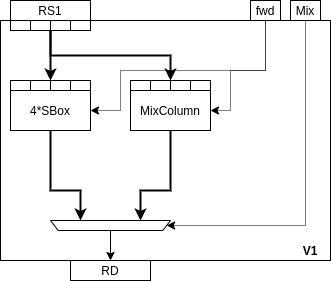
\includegraphics[width=\textwidth]{diagrams/ise-datapath-v1.png}
    \caption{\ISE{1}}
    \label{fig:design:fu_block:v1}
\end{subfigure}
\begin{subfigure}[t]{0.40\textwidth}
    \centering
    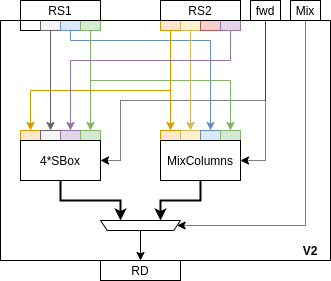
\includegraphics[width=\textwidth]{diagrams/ise-datapath-v2.png}
    \caption{\ISE{2}}
    \label{fig:design:fu_block:v2}
\end{subfigure}

\begin{subfigure}[t]{0.40\textwidth}
    \centering
    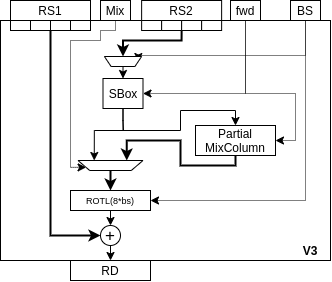
\includegraphics[width=\textwidth]{diagrams/ise-datapath-v3.png}
    \caption{\ISE{3}}
    \label{fig:design:fu_block:v3}
\end{subfigure}
\begin{subfigure}[t]{0.40\textwidth}
    \centering
    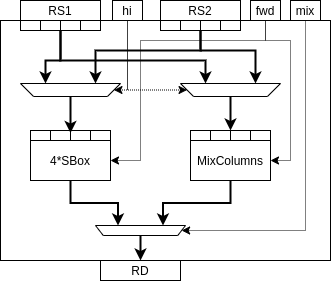
\includegraphics[width=\textwidth]{diagrams/ise-datapath-v5.png}
    \caption{\ISE{5}}
    \label{fig:design:fu_block:v5}
\end{subfigure}

\caption{
Micro-architecture block diagrams for the AES functional units, for
each ISE variant.
}
\end{figure}

